Before implementing own solution, let's firstly uncover some available and current solutions to this very problem. Naturally, big progress and research is performed in this topic, therefore this chapter is not meant to provide full market scan, or list every solution available. It rather aims to discover some fine examples of neural network implementations which perform well.

Later on you'll stumble upon a list of available face recognition databases and data sets which can be used for training and evaluating the very own implementation. Each of the data set description is accompanied by a short list of their respective metrics.

\section{Existing implementations}

There are many available solution and existing implementations. Their implementations naturally differs, models compete and cover different use cases. We've already established, that the face recognition is dynamic field with competitive nature. Open challenges and competitions are enabling greater progress in the field. However that makes it impossible to provide always up to date review of available solutions and implementations.

Here's a short list of example challenges and competitions held in face recognition field. It provides insight how wide the field is and how many different architectures can be used:
\begin{itemize}
    \item MSCeleb challenges\,\footnote{\url{https://www.msceleb.org/celeb1m/1m} and \url{https://www.msceleb.org/challenge2/2017}}
    \item Deep learning benchmark\,\footnote{\url{https://github.com/u39kun/deep-learning-benchmark}}
    \item NIST: Fusion of Face Recognition Algorithms 2018\,\footnote{\url{https://www.nist.gov/programs-projects/fusion-face-recognition-algorithms-2018}}
    \item Surveillance Face Recognition Challenge\,\cite{sur_challenge}
\end{itemize}

Therefore let's rather focus one solution and pick some details of its design to better understand how such solution is made and what does it mean.

\subsection{FaceNet}

This state-of-the-art solution backed by Google\,\cite{facenet} is one of the leading solutions in the field. Its implementation is open source\,\footnote{\url{https://github.com/davidsandberg/facenet}} including pre-trained models. FaceNET is focused on the same kind of input data as this thesis, therefore it is really great example of an existing solution to discover. It is inspired by proposed implementations of Visual Geometry Group, University of Oxford\,\cite{vgg_face_reco}.

FaceNET is a CNN based solution. It operates in multiple steps. At first it locates a face on given image by using multi-task cascaded convolutional network\,\cite{mtcnn}. Then it builds a face identification network using multiple architectures. It provides models for \textbf{Inception ResNet} and \textbf{SqueezeNet} architectures.

\subsection{ResNet}

Older architecture of CNN provides reliable solution for image classification\,\cite{resnet}. This architecture is mainly accented in Google AI workshop. It's a certainly complex architecture,\ref{fig:resnet} producing models of many parameters and great size, therefore it might not be very useful in use cases with limited resources.

\begin{figure}[ht]
    \centering
    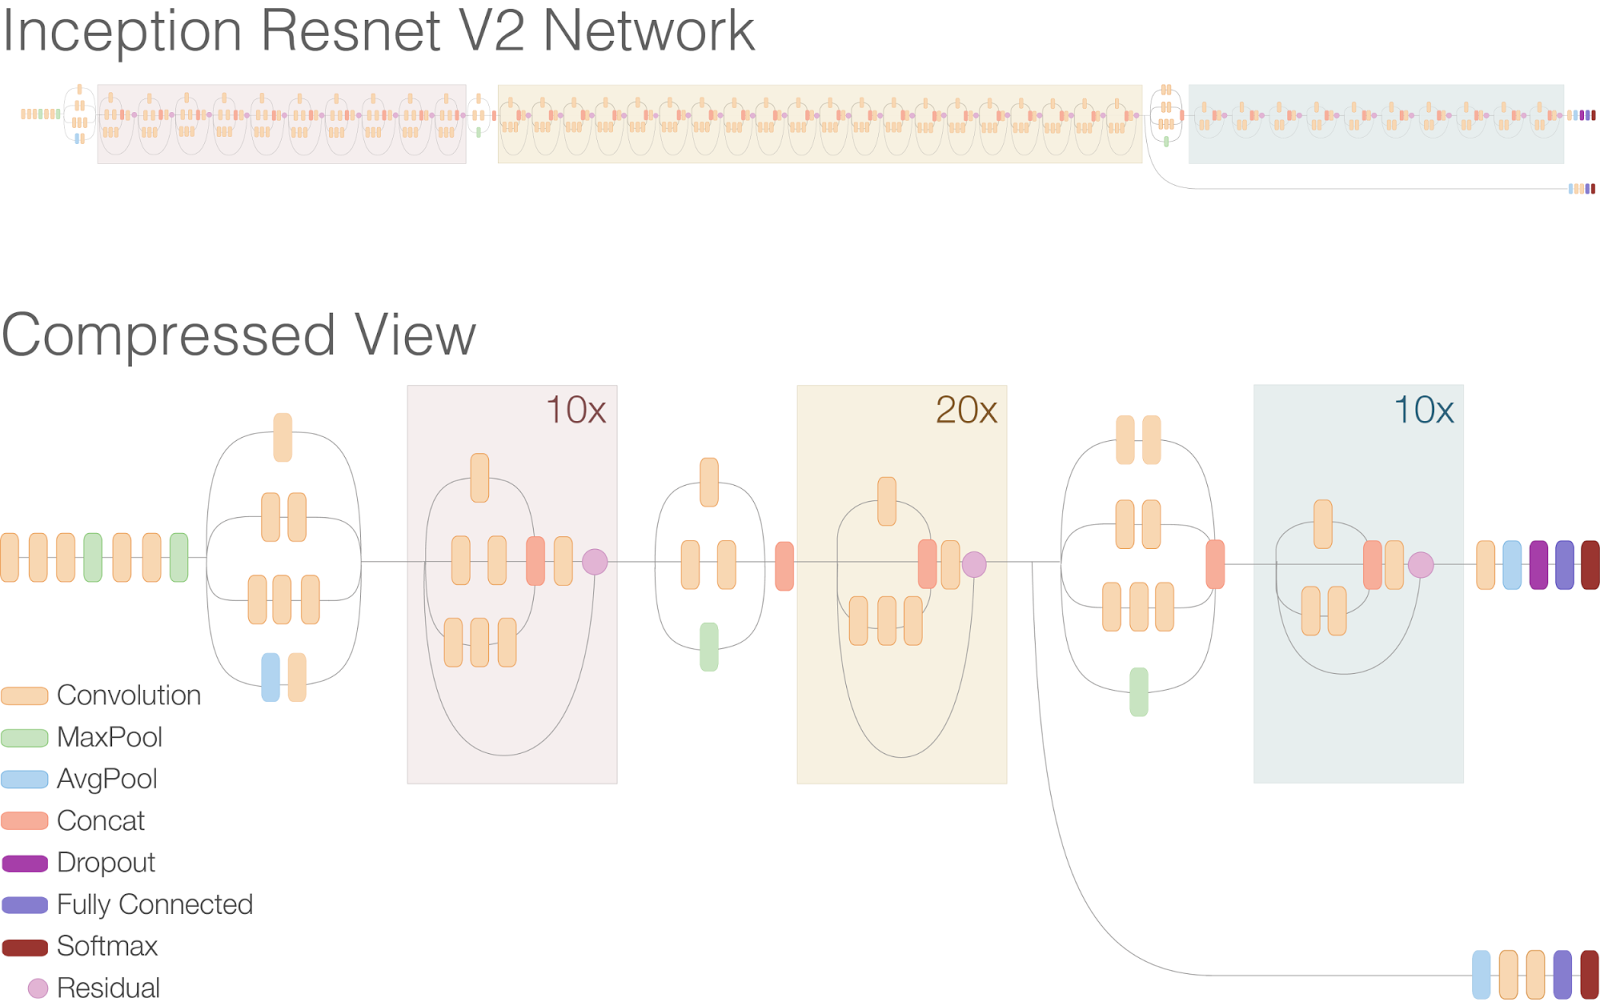
\includegraphics[width=.8\textwidth]{obrazky-figures/resnet.png}
    \caption{ResNet model structure}
    \label{fig:resnet}
\end{figure}

\subsection{SqueezeNet}

SqueezeNet\,\cite{squeezenet} is not a direct application as the previous mention. It's rather an architecture of deep neural networks. It introduced itself as an network with AlexNet accuracy, despite having half of the amount of parameters. It's designed to create small networks with fewer parameters than any other common network type.

Initially this network was released in 2016 as a Caffe implementation. Later it found its way into other frameworks and was hugely adopted in use cases with limited resources. Therefore it makes applications, which would require a model to be run on low-powered processing platforms like FPGAs and smartphones, available.

It is capable of optimizations like \textit{Deep Compression}\,\cite{compression}, which allows trained models to be compressed. In case of SqueezeNet it can reduce model size $10\times$.

\section{Frameworks}

Each of the previously mentioned solutions has something in common. They've used a AI framework or library of some sort. Writing neural networks from scratch is obviously a complex task, therefore there are many initiatives which seeks to simplify and facilitate access to such complex structures. Let§s list some most common ones and list some of their basic advantages and disadvantages.

\subsection{Torch and PyTorch}

Torch is a deep-learning and computational framework written in Lua. While very powerful, its design prevented from being adopted by users and researchers. The main problem was in usage of rather exotic programming language which created barrier for users. It's been decided to create a Python clone of the framework, which brought PyTorch\,\footnote{\url{https://pytorch.org/}} to existence. It was created by Facebook and released in 2007 under an open source license. One of it's key features are dynamic computation graphs, which can serve well when processing inputs or outputs of variable length.

\begin{itemize}
    \item[$\boldsymbol{+}$] Many pluggable modules
    \item[$\boldsymbol{+}$] Easy to integrate different extensions
    \item[$\boldsymbol{+}$] Simple to define own layers
    \item[$\boldsymbol{+}$] Straightforward access to running code on GPU
    \item[$\boldsymbol{+}$] Offers dynamic computation graphs
    \item[$\boldsymbol{+}$] Broad community and wide audience
    \item[$\boldsymbol{+}$] Easier to inspect and monitor training of models
    \item[$\boldsymbol{+}$] Intuitive API
    \item[$\boldsymbol{-}$] Requires custom training code
\end{itemize}

\subsection{Tesorflow}

This library created by Google was designed as a replacement for their previous project called Theano. Tensorflow\,\footnote{\url{https://www.tensorflow.org/}} a heavyweight framework written as a Python API in C/C++. It simplifies researcher's task in many ways better than other frameworks. For example it generates a computational graph and performs automatic differentiation. That means the user is not required to write a training code (backpropagation) every time, he's experimenting with a new network topology. Since this framework is backed by Google it thrives in many different applications and can scale across devices. Many possibilities for applying saved models in different environment enables use of AI in mobile devices and even in web browsers. However it's broad possibilities and options make this framework hard to understand and for newcomers it can be confusing and too complex. Therefore an abstraction layer above Tensorflow had been created, but more about that in the Keras subsection below.

\begin{itemize}
    \item[$\boldsymbol{+}$] Native Python and Numpy integration
    \item[$\boldsymbol{+}$] Automatic training code
    \item[$\boldsymbol{+}$] Broad community and wide audience
    \item[$\boldsymbol{-}$] Heavyweight frameworks
    \item[$\boldsymbol{-}$] A bit slower than PyTorch
\end{itemize}

\subsection{Caffe and Caffe2}

Caffe is another competition framework, which is widely popular among researchers. It started as a C/C++ port of Matlab's implementation of fast convolutional networks. It's mainly oriented on feed forward networks and image processing and is not intended for other deep learning application like text processing or 1D series data. Later on it became performance wise obsolete and community of Caffe developers decided to start from scratch and created a long-awaited successor Caffe2\,\footnote{\url{https://caffe2.ai/}}. Backed by Facebook as their second deep learning toolkit after PyTorch it provides more lightweight and scalable solution than before. It's main area of focus is enterprise grade production environments.

\begin{itemize}
    \item[$\boldsymbol{+}$] Great for image processing and feedforward networks
    \item[$\boldsymbol{+}$] Automatic training code
    \item[$\boldsymbol{+}$] Lightweight
    \item[$\boldsymbol{+}$] BSD license
\end{itemize}

\subsection{Keras}

A modern abstraction layer above Tensorflow. Authors and users of Tensorflow suffered from heavy and complex code structures and when PyTorch appeared with their light and straightforward Python API, they've started adopting the same principals for the Tensorflow as well. Therefore a project named Keras\,\footnote{\url{https://keras.io/}} was created. It provides intuitive API inspired by Torch and while starting from Tensorflow it outgrown this base and spread across many deep learning libraries as its back eds - Theano, Deeplearning4j, and CNTK. In addition to its high level abstraction over the back ends Keras also provides means to drill down and optimize and manipulate the underlying code.

\begin{itemize}
    \item[$\boldsymbol{+}$] Intuitive API
    \item[$\boldsymbol{+}$] Multiple back ends to choose from
    \item[$\boldsymbol{+}$] Lightweight
    \item[$\boldsymbol{+}$] Fast growing community
    \item[$\boldsymbol{+}$] Recognized as a standard Python API for neural networks
\end{itemize}

\section{Data Sets}

In order to better understand the nature of CCTV imagery, pictures in the wild and the source data we are about to work with, let's describe some commonly used databases of face images and face recognition data. It's crucial to understand the variety and differences between subjects captured on sample images, like their age, sex, and ethnicity. Also we need to pay attention to circumstances of the photo setup. That means for example consistency of resolution across samples, poses and angles, etc.

\subsection{FDDB: Face Detection Data Set and Benchmark}

This data set provides annotations for Faces in the Wild\,\cite{fiw} database. FDDB\,\cite{fddb} lists coordinates for bounding boxes of over 5 thousands faces located on pictures from Faces in the Wild database. Usually multiple faces are located on a single picture. This data set can provide ground for face detection algorithm and therefore it can be benefited from in the first step of implementation. For recognition of individuals whom such face belongs to, another data set has to be used. A great accompanying data set can be the LFW mentioned in next subsection.

\begin{table}[ht]
    \centering
    \caption{FDDB data set metrics}

    \begin{tabularx}{0.75\textwidth}{l|l}
        \toprule
        Number of subjects & \num{5171} \\
        Total images &  \num{28045} \\
        Poses & Varies \\
        Resolution & All kind, even blurred faces \\
        \bottomrule
    \end{tabularx}
\end{table}

\subsection{LFW: Labeled Faces in the Wild}

LFW\,\cite{lfw} provides labels for images from Faces in the Wild data set mentioned before. Therefore when used in conjunction with FDDB, this data set can provide a robust base for face recognition. The database spans many identities, though it lacks volume\,--\, many subjecs have only one image in the data set. That does not provide enough coverage to train a network to recognize that individual.

\begin{table}[ht]
    \centering
    \caption{LWF data set metrics}

    \begin{tabularx}{0.75\textwidth}{l|l}
        \toprule
        Number of subjects & \num{5749} \\
        Total images & \num{13233} \\
        Samples per subject & Varies, many have just one, others up to 40 \\
        Resolution & 250 $\times$ 250 \\
        License & Creative Commons \\
        \bottomrule
    \end{tabularx}
\end{table}

\subsection{The Extended Yale Face Database B}

Extended version of original Yale Face Database. The extension was provided by UCSD\,\cite{ext_yale_paper}. This database comprises over \num{16000} images of 28 unique subjects. They are fitted to same size and resolution, covering various angles of the face. There are 9 poses provided for each person, each of them covering 64 different illumination condition.  When compared to a large scale data set this database lacks volume, however it maintains consistency across its samples.

\begin{table}[ht]
    \centering
    \caption{Extended Yale Face Database B metrics}

    \begin{tabularx}{0.75\textwidth}{l|l}
        \toprule
        Number of subjects & 28 \\
        Total images & \num{16128} \\
        Samples per subject & 576 \\
        Poses & 9 \\
        Resolution & $168 \times 192$ pixels \\
        License & Free to use for research purposes\\
        \bottomrule
    \end{tabularx}
\end{table}

\subsection{SCface - Surveillance Cameras Face Database}

A face database originate from University of Zagreb. Quality data set of surveillance like face images. It aims to simulate a CCTV captured images by simulating an uncontrolled indoor environment. Each of 130 subjects is captured by up to 8 video surveillance cameras. Some of them even capable of IR capturing. Each camera produces images of different resolution and sharpness. Cameras are also set in different angles against the subject. SCFace\,\cite{scface} mimics real-world circumstances and use cases of CCTV, therefore this data set can be used to train robust solutions for face recognition targeting CCTV and surveillance cameras.

A disadvantage is the size of this data set, where we can find \num{4160} image samples only. When compared to large-scaled data set like the VGGFace and VGGFace2 mentioned in next subsection, this data set lacks volume. Also the variety of subjects is not robust enough in comparison to other data set. As said, SCFace captures 130 subjects. Most of them are of the same sex, all of the same ethnicity.

\begin{table}[ht]
    \centering
    \caption{SCFace data set metrics}

    \begin{tabularx}{0.75\textwidth}{l|l}
        \toprule
        Number of subjects & 130 \\
        Total images & \num{4160} \\
        Samples per subject & Fixed amount of 32 images per person \\
        Resolution & Varies, 3 different sizes \\
        License & Custom \\
        \bottomrule
    \end{tabularx}
\end{table}

This database is available for research purposes and upon written request to the authors.

\subsection{VGGFace2}

Visual Geometry Group produced a second iteration of their face recognition data set\,\cite{VVGFace2}. This is one of the most wide data sets which are publicly available. It provides a wide-scale data for face recognition for over 9000 different identities. Distribution of individuals varies though, with minimal 87 images up to 843 per identity. Average number of images per subject is 362. The data set contains over \num{3.3} milion of images. Subjects varies in ethnicity, age and profession, while the images varies in angles or poses.

The data set is made available under Creative Commons license\,\footnote{\url{https://creativecommons.org/licenses/by-sa/4.0/}}, therefore it's available for broad use to any project.

\begin{table}[ht]
    \centering
    \caption{VGGFace2 data set metrics}

    \begin{tabularx}{0.75\textwidth}{l|l}
        \toprule
        Number of subjects & \num{9294} \\
        Total images & \num{3311286} \\
        Samples per subject & Varies, 87--843 per subject \\
        Resolution & Varies, many different sizes \\
        License & Creative Commons \\
        \bottomrule
    \end{tabularx}
\end{table}

This project also provides sample models trained on this data set. However, the example pre-trained neural network models provided within this project are not the sole example of the data set usage. Many popular face recognition models are trained on this data set. For example FaceNET can be seen as one of the popular projects which benefits from this data set.

\subsection{MSCeleb}

This data set is provided by Microsoft company and various challenges and competitions were held against it. Similarly to the previous one, MSCeleb\,\cite{msceleb} is a large scale data set, though oriented specifically on celebrities. Each challenge announced by researcher team behind this dataset is backed by a specific subset of the data set. These selections are usually oriented of certain aspects of face recognition, therefore can be proven valid for use case covered in this thesis.

Subjects vary in all desired aspects and images provide enough variety in poses and background noise.

\begin{table}[ht]
    \centering
    \caption{MSCeleb data set metrics}

    \begin{tabularx}{0.75\textwidth}{l|l}
        \toprule
        Number of subjects & \num{99892} \\
        Total images & \num{8456240} \\
        Samples per subject & Varies, average 85 per entity \\
        Resolution & Varies, up to 300 $\times$ 300 \\
        License & Research purposes only \\
        \bottomrule
    \end{tabularx}
\end{table}

\subsection{CelebA}

CelebA\,\cite{celeba} is another large scale database of faces. The focus is on celebrities faces, the same as in the MSCeleb dataset. Pictures cover wide variety of poses and background noises. Each image is provided with 5 landmarks locations and 40 binary attributes.

Subjects vary in ethnicity, age, sex as well as in appearance. Data set includes faces with facial hair, poses and with different emotions.

\begin{table}[ht]
    \centering
    \caption{CelebA data set metrics}

    \begin{tabularx}{0.75\textwidth}{l|l}
        \toprule
        Number of subjects & \num{10177} \\
        Total images & \num{202599} \\
        Samples per subject & Varies \\
        Resolution & Varies \\
        License & Research purposes only \\
        \bottomrule
    \end{tabularx}
\end{table}
